% ===========================================================================
%  Foundation-Model-Based Depth Completion for Volumetric Environment
%  Modelling on an Assistive Mobile Manipulator
%
%  DRAFT v0.1 -- 2026-11-24
%  Compile with: pdflatex main && bibtex main && pdflatex main && pdflatex main
%  (or upload the folder to Overleaf). Figures are placeholders, see \figph.
% ===========================================================================
\documentclass[conference]{IEEEtran}

\usepackage{cite}
\usepackage{amsmath}
\usepackage{newtxtext,newtxmath}
\usepackage{graphicx}
\usepackage{booktabs}
\usepackage{multirow}
\usepackage{xcolor}
\usepackage{tikz}
\usetikzlibrary{positioning,arrows.meta,fit,calc}
\usepackage{url}
\usepackage[hidelinks]{hyperref}

% ---------------------------------------------------------------- macros
\newcommand{\todo}[1]{\textcolor{red}{[TODO: #1]}}
% Figure placeholder: \figph{<height>}{<what the figure should show>}
\newcommand{\figph}[2]{%
  \fbox{\parbox[c][#1][c]{0.95\linewidth}{\centering\footnotesize
  \textbf{[Figure placeholder]}\\[2pt]#2}}}
\newcommand{\figphwide}[2]{%
  \fbox{\parbox[c][#1][c]{0.97\textwidth}{\centering\footnotesize
  \textbf{[Figure placeholder]}\\[2pt]#2}}}

\newcommand{\R}{\mathbb{R}}
\newcommand{\Dm}{Z}            % measured depth
\newcommand{\Dp}{M}            % MoGe prediction
\newcommand{\Om}{\Omega}       % valid measurement set
\DeclareMathOperator*{\median}{median}
\DeclareMathOperator*{\argmin}{arg\,min}

\begin{document}

\title{Metric Monocular Priors for Depth Completion in\\
Volumetric Environment Modelling of an\\
Assistive Mobile Manipulator}

\author{%
\IEEEauthorblockN{Simon Spielmann}
\IEEEauthorblockA{Institute of Robotics and Mechatronics\\
German Aerospace Center (DLR)\\
Wessling, Germany}
\and
\IEEEauthorblockN{Claude}
\IEEEauthorblockA{Anthropic\\
San Francisco, CA, USA}
}

\maketitle

% =========================================================================
\begin{abstract}
Time-of-flight RGB-D cameras are the standard exteroceptive sensor for
close-range manipulation, yet their depth images routinely miss
\(20\)--\(30\,\%\) of the pixels on dark, specular, transparent or
grazing-angle surfaces and at depth discontinuities. When such images are
fused into a volumetric map, these holes become \emph{unknown} space, which
downstream collision checkers commonly treat as free. We present the
perception-to-mapping pipeline of a wheelchair-mounted assistive manipulator
that addresses this problem with four stages: (i)~a depth completion stage
that aligns the metric monocular geometry foundation model MoGe-2 to the sensor
measurements, (ii)~a kinematic self-filter that removes the robot arm,
(iii)~a pose-based human filter, and (iv)~GPU-accelerated TSDF integration
with nvblox, which accumulates the per-frame observations over time into a
stable environment model. The core contribution is the depth filler, for
which we derive and compare two alignment schemes: a closed-form local affine
alignment in the spirit of the guided filter, and an edge-aware,
measurement-weighted variational correction of the log-depth solved by
preconditioned conjugate gradients. Both were tuned in deterministic
parameter sweeps over roughly \(800\) configurations on real robot data. On
held-out sensor measurements, the tuned local affine scheme reaches
\(2.75\,\%\) AbsRel (\(3.6\,\)cm MAE) and the variational scheme
\(3.27\,\%\) (\(4.1\,\)cm), both about four times better than global scale
alignment (\(12.8\,\%\)). However, we show that the holdout metric
systematically favours the local scheme. In regions with little surrounding
measurement support, the local scheme falls back to the global scale and
produces visible spatial seams and frame-to-frame jumps, whereas the
variational scheme produces a correction field that is continuous by
construction and decays smoothly away from the measurements. We therefore use
the variational scheme in the mapping pipeline.
\end{abstract}

\begin{IEEEkeywords}
Depth completion, monocular depth estimation, foundation models, RGB-D
sensing, TSDF mapping, self-filtering, assistive robotics.
\end{IEEEkeywords}

% =========================================================================
\section{Introduction}
\label{sec:intro}

Assistive mobile manipulators operate in cluttered domestic environments, in
close proximity to their user and to bystanders. To plan collision-free arm
motions, they need a dense and up-to-date geometric model of their
surroundings. On our platform, the wheelchair-based assistive robot MAYA with
a 7-DoF arm (the software also supports its predecessor
EDAN~\cite{vogel2020edan}), this model is built
from a single platform-mounted Azure Kinect time-of-flight (ToF)
camera~\cite{tolgyessy2021kinect}. The resulting map is consumed by an
octree-based collision checker~\cite{pan2012fcl,carpentier2019pinocchio}.

ToF depth images are accurate where they are valid. Where they are not, they
are simply empty. In the recordings used in this paper, \(28\,\%\) of the
pixels of the color-registered depth image carry no measurement. These holes
are not randomly distributed. They cluster on black and glossy surfaces such
as monitors, chair legs and furniture fronts, on glass, at grazing angles, at
the boundary between the ToF and color fields of view, and along depth
discontinuities where multipath and mixed pixels are rejected. These are
exactly the structures a manipulator is likely to collide with.

The way the volumetric map treats such holes is critical. A TSDF
integrator~\cite{curless1996volumetric,newcombe2011kinectfusion,millane2024nvblox}
only updates voxels along rays with a valid measurement, so a hole leaves the
corresponding voxels \emph{unobserved}. Our occupancy extraction, like many
practical collision pipelines that must avoid blocking the robot on every
unseen voxel, classifies unobserved space as free (Sec.~\ref{sec:nvblox}). A
persistent sensor hole on a black table edge therefore becomes a persistent
gap in the collision model.

Recent monocular geometry foundation
models~\cite{ranftl2020midas,yang2024depthanything,yang2024depthanythingv2,piccinelli2024unidepth,hu2024metric3dv2,bochkovskii2025depthpro,wang2025moge,wang2025moge2}
predict dense, sharp depth from a single RGB image, including on surfaces
where active sensing fails. MoGe-2~\cite{wang2025moge2} additionally
predicts \emph{metric} scale and accepts the true camera field of view. Its
raw output is nevertheless not accurate enough to be used in place of
measured depth: a single global scale correction leaves a mean relative error
of \(12.8\,\%\) on our data (Sec.~\ref{sec:exp}). The prediction must
therefore be aligned locally to the sensor wherever measurements exist, while
behaving sensibly where they do not.

\textbf{Contributions.} This paper makes the following contributions:
\begin{enumerate}
  \item A complete, real-time perception-to-mapping pipeline
        (camera \(\rightarrow\) MoGe depth filler \(\rightarrow\) arm
        self-filter \(\rightarrow\) human filter \(\rightarrow\) nvblox) for
        an assistive mobile manipulator, including the timestamp
        synchronisation between images, odometry and joint states
        (Sec.~\ref{sec:system}).
  \item Two alignment schemes that turn a metric monocular prediction into a
        hole filler that preserves the measurements: a closed-form
        \emph{local affine} alignment (Variant~A) and an edge-aware
        \emph{variational log-depth correction} (Variant~B), together with a
        GPU implementation of the latter (Sec.~\ref{sec:filler}).
  \item A deterministic, reproducible tuning protocol based on block-wise
        holdout of real sensor measurements, and its results on approximately
        \(800\) configurations (Sec.~\ref{sec:exp}).
  \item An analysis showing that the holdout metric is biased towards local
        methods, and that Variant~A becomes spatially and temporally unstable
        when measurement support around a hole is low. This motivates
        Variant~B for map building, even though it scores lower on the holdout
        metric (Sec.~\ref{sec:discussion}).
\end{enumerate}

% =========================================================================
\section{Related Work}
\label{sec:related}

\textbf{Monocular depth estimation.}
Learning-based monocular depth estimation has evolved from scene-specific
regressors~\cite{eigen2014depth} to zero-shot models trained on large data
mixtures. MiDaS~\cite{ranftl2020midas} and Depth
Anything~\cite{yang2024depthanything,yang2024depthanythingv2} predict
affine-invariant (relative) depth, which requires a per-image scale and
shift. A second generation of models predicts metric depth directly by
conditioning on, or estimating, camera intrinsics.
Examples are UniDepth~\cite{piccinelli2024unidepth},
Metric3D\,v2~\cite{hu2024metric3dv2} and Depth Pro~\cite{bochkovskii2025depthpro}.
MoGe~\cite{wang2025moge} predicts an affine-invariant point map with a robust,
optimal-alignment training objective. MoGe-2~\cite{wang2025moge2} extends it
to metric scale and sharper detail. We build on MoGe-2 because it (i)~accepts
the known horizontal field of view, which removes the focal-length ambiguity,
(ii)~produces a validity mask for sky and undefined regions, and (iii)~offers
a token-count parameter that trades detail for latency.

\textbf{Depth completion.}
Classical depth completion propagates sparse or semi-dense measurements under
image guidance, for example by joint bilateral or guided
filtering~\cite{he2013guided}, or by optimisation-based propagation with
affinities derived from color~\cite{levin2004colorization,barron2016bilateral}.
Learned approaches regress dense depth from RGB and sparse
depth~\cite{uhrig2017sparsity,ma2018sparse,park2020nlspn}. Zhang and
Funkhouser~\cite{zhang2018deepcompletion} complete RGB-D images by predicting
surface normals and occlusion boundaries from color and then solving a global
optimisation. This decouples the learned geometry from the measured scale, a
principle we share. Prompt Depth Anything~\cite{lin2025promptda} conditions a
depth foundation model on a low-resolution metric prompt. Diffusion-based
completion such as Marigold-DC achieves high quality but needs seconds per
frame. ClearGrasp~\cite{sihan2019transparent}
targets the transparent-object failure mode specifically. In contrast to
learned completion networks, our filler requires no training on the target
sensor. It combines a frozen foundation model with a lightweight, analytically
understood alignment stage, and it never modifies a valid measurement.

\textbf{Volumetric mapping.}
TSDF fusion~\cite{curless1996volumetric} was popularised for RGB-D cameras by
KinectFusion~\cite{newcombe2011kinectfusion} and adapted to robotics by
Voxblox~\cite{oleynikova2017voxblox} and its GPU successor
nvblox~\cite{millane2024nvblox}. Probabilistic occupancy maps such as
OctoMap~\cite{hornung2013octomap} are an alternative. All of them accumulate
evidence over time, which suppresses per-frame noise but also stores
erroneous observations persistently. This makes the
quality of filled depth and the handling of dynamic objects first-order
concerns. Dedicated dynamic-object detection in volumetric maps has been
studied, for example, in Dynablox~\cite{schmid2023dynablox}. We take the
simpler route of masking humans in image space before integration.

% =========================================================================
\section{System Overview}
\label{sec:system}

\begin{figure*}[t]
\centering
\resizebox{\textwidth}{!}{%
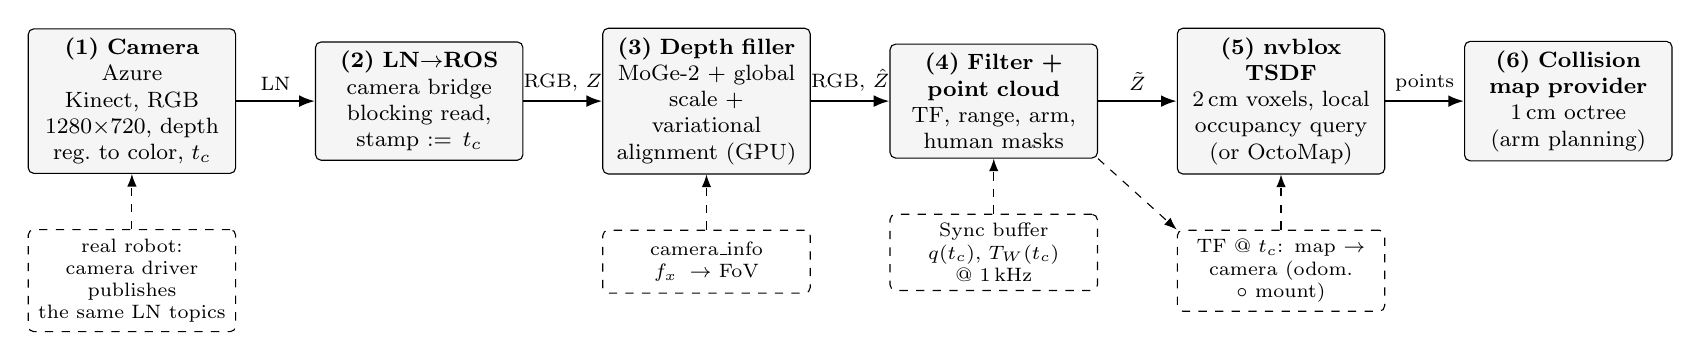
\begin{tikzpicture}[
  node distance=4mm and 10mm,
  blk/.style={draw, rounded corners=2pt, align=center, font=\footnotesize,
              minimum height=11mm, text width=24mm, fill=gray!8},
  aux/.style={draw, dashed, rounded corners=2pt, align=center,
              font=\scriptsize, text width=24mm, minimum height=8mm},
  arr/.style={-{Latex[length=2mm]}, thick},
  darr/.style={-{Latex[length=1.6mm]}, dashed}]
  \node[blk] (cam) {\textbf{(1) Camera}\\Azure Kinect, RGB\\\(1280{\times}720\), depth\\reg.\ to color, \(t_c\)};
  \node[blk, right=of cam] (brg) {\textbf{(2) LN\(\rightarrow\)ROS}\\camera bridge\\blocking read,\\stamp \(:=t_c\)};
  \node[blk, right=of brg] (moge) {\textbf{(3) Depth filler}\\MoGe-2 + global\\scale + variational\\alignment (GPU)};
  \node[blk, right=of moge] (flt) {\textbf{(4) Filter +}\\\textbf{point cloud}\\TF, range, arm,\\human masks};
  \node[blk, right=of flt] (nvb) {\textbf{(5) nvblox TSDF}\\2\,cm voxels, local\\occupancy query\\(or OctoMap)};
  \node[blk, right=of nvb] (col) {\textbf{(6) Collision}\\\textbf{map provider}\\1\,cm octree\\(arm planning)};
  \draw[arr] (cam) -- node[above,font=\scriptsize]{LN} (brg);
  \draw[arr] (brg) -- node[above,font=\scriptsize]{RGB, \(Z\)} (moge);
  \draw[arr] (moge) -- node[above,font=\scriptsize]{RGB, \(\hat Z\)} (flt);
  \draw[arr] (flt) -- node[above,font=\scriptsize]{\(\tilde Z\)} (nvb);
  \draw[arr] (nvb) -- node[above,font=\scriptsize]{points} (col);
  \node[aux, below=7mm of cam] (drv) {real robot:\\camera driver publishes\\the same LN topics};
  \node[aux, below=7mm of moge] (info) {camera\_info\\\(f_x \rightarrow\) FoV};
  \node[aux, below=7mm of flt] (sync) {Sync buffer\\\(q(t_c)\), \(T_{W}(t_c)\) @ 1\,kHz};
  \node[aux, below=7mm of nvb] (tf) {TF @ \(t_c\): map \(\rightarrow\)\\camera (odom.\ \(\circ\) mount)};
  \draw[darr] (drv) -- (cam);
  \draw[darr] (info) -- (moge);
  \draw[darr] (sync) -- (flt);
  \draw[darr] (flt.south east) -- (tf.north west);
  \draw[darr] (tf) -- (nvb);
\end{tikzpicture}}
\caption{Software architecture of the perception-to-mapping pipeline. Each
block is a separate process. (1)~runs only with a locally attached camera; on
the robot, the camera driver publishes the same LN topics. From (2) on, stages
communicate over ROS\,2 topics, and every message of a frame carries the
capture timestamp \(t_c\) as its header stamp. Solid arrows: image data flow at
camera rate (15\,Hz). Dashed: auxiliary state. Pixels removed by the filters in
(4) are set to zero (``no measurement''). nvblox does not integrate zero
pixels, so masked regions neither add nor carve geometry.}
\label{fig:architecture}
\end{figure*}

Fig.~\ref{fig:architecture} shows the pipeline. Each stage runs as its own
process. Robot-internal state (odometry, joint angles, camera mount) is
obtained through the robot's real-time middleware, links\_and\_nodes (LN).
Sec.~\ref{sec:architecture} explains why the pipeline is split this way.
The remaining sections describe the stages in data-flow order. The depth
filler is the focus of Sec.~\ref{sec:filler}.

\subsection{Software Architecture and Design Decisions}
\label{sec:architecture}
The pipeline consists of six stages, each with a single task:
(1)~a camera publisher that reads a locally attached Azure Kinect and
publishes RGB, registered depth and intrinsics with the capture timestamp on
LN; (2)~a bridge that forwards these LN topics unchanged to ROS\,2;
(3)~the depth filler (Sec.~\ref{sec:filler}); (4)~a filter node that
publishes the camera pose as TF, applies the range, arm and human filters
(Secs.~\ref{sec:selffilter} and~\ref{sec:humanfilter}) and publishes the
filtered depth image and point cloud; (5)~the volumetric map
(Sec.~\ref{sec:nvblox}); and (6)~a collision-map provider that converts the
map into a collision octree for the arm planner. The design follows from
the decisions below.

\textbf{ROS\,2 as the data bus.} All image data between the stages travels over
ROS\,2. ROS provides native message types for everything that flows through
the pipeline: images, camera intrinsics, point clouds, transforms and octrees.
nvblox, OctoMap~\cite{hornung2013octomap} and exact time synchronisation of
topics work directly with these types. Every intermediate result can also be
shown in RViz without extra code, such as raw and completed depth next to
each other, the filtered point cloud or the map. This made debugging the filler
and the masks much easier. LN remains where the robot already uses it: the
camera driver, the synchronisation buffer, the camera mount and the map-reset
services.

\textbf{One process per task.} An earlier version did camera access, bridging,
filtering, TF and point-cloud generation in one timer loop. Splitting it has
three advantages. First, the stages have conflicting dependencies. The
filler needs a PyTorch environment for MoGe, while the other stages need the
robot middleware and the system ROS packages. Separate processes that talk
over ROS avoid this conflict. Second, a slow stage cannot block a fast one.
The filler's latency does not delay the camera stream, and the
camera does not wait for the filler. Third, stages can be swapped or
skipped. The filter node can read the raw instead of the completed depth, and
nvblox can be replaced by OctoMap. Neither change touches any other stage.

\textbf{Identical input on the robot and in the lab.} On the robot, the camera
driver already publishes RGB, depth and intrinsics on LN. Stage~(1) publishes
exactly the same topics and message definitions from a locally attached
camera. Everything from stage~(2) on is therefore identical in both setups,
and the bridge needs only a single input path. Because the LN read blocks
until the next packet arrives, the bridge needs no timer and forwards every
frame as soon as it arrives.

\textbf{The capture timestamp is passed through.} Stage~(1) stamps each frame
with its capture time \(t_c\). This is the same clock that the synchronisation
buffer uses (Sec.~\ref{sec:sync}). The bridge writes \(t_c\) into the header
stamp, and no later stage changes it. The filler copies the header of its
input, and the filter node stamps the TF, the filtered depth and the point
cloud with it. This has two consequences. The filter node finds the joint
angles and odometry of exactly this frame in the buffer, even though the
filler adds about \(100\,\)ms of latency. Without this, the arm mask would lag
behind a moving arm. The map also finds, through TF, the camera pose of exactly
this frame. Because colour, depth and intrinsics of one frame carry the
identical stamp, all consumers synchronise them exactly rather than
approximately.

\textbf{Newest frame first.} The filler is slower than the camera. It keeps
only the newest synchronised frame and drops older ones, so that latency
cannot grow without bound. It republishes colour and intrinsics together with
the completed depth. Downstream nodes therefore receive a consistent triple
with a single stamp.

\textbf{Fill first, then filter.} The range, arm and human filters run after
the filler (Sec.~\ref{sec:humanfilter}). MoGe sees the full image, which
helps its scale estimate. Anything that was filled into a masked region is
removed afterwards. The range limit therefore also applies to filled values.

\textbf{TF from the filter node.} The filter node already queries the
synchronisation buffer for the arm filter. It therefore also publishes
\(T_{\text{map},W_t}(t_c)\) together with the static camera mount, before
the filtered depth of the same frame.

\textbf{Depth image for nvblox, point cloud for the rest.} The nvblox
PyTorch interface integrates depth images by projection. The filter node
therefore publishes the same filtered data twice: as a depth image for nvblox
and as a point cloud for OctoMap and RViz. The collision-map provider subscribes to whichever map backend is
active. It turns the occupied points into a COAL octree, axis-aligned boxes
or a prepared map for the collision checker, and can remove a grasped
object's volume from the map.

\subsection{Sensing and Pre-Processing}
\label{sec:sensor}
The Azure Kinect runs at \(15\,\)Hz with \(720\)p color and the wide
field-of-view, \(2{\times}2\)-binned depth mode. Depth is re-projected into
the color camera with the factory calibration, so that RGB and depth share
the intrinsics \(K\) and are pixel-aligned. Depth values beyond
\(8\,\)m are discarded in the filter stage, after filling. A value of \(0\) denotes ``no measurement'' throughout
the pipeline.

\subsection{Time Synchronisation}
\label{sec:sync}
Both the self-filter and the map integration need the robot state at the
exposure time of the image, not at processing time. Otherwise, arm motion
during a \(\sim\!100\,\)ms processing delay would shift the self-filter mask
by several centimetres. A dedicated synchronisation service samples the
platform odometry \(T_{W_s W_t}(t)\) and the joint configuration \(q(t)\) at
\(1\,\)kHz into a lock-protected ring buffer of \(3000\) slots (\(3\,\)s). The
buffer consists of at most two time-sorted segments, so a query for the
sample closest to the image timestamp is a single comparison followed by a
binary search, \(\mathcal{O}(\log n)\), without copying. A fill thread and a
service thread are separated so that queries never starve the buffering.

% =========================================================================
\section{MoGe-Based Depth Filler}
\label{sec:filler}

\subsection{Design Rationale and Evolution}
\label{sec:evolution}
The filler went through several iterations, which we summarise because they
explain its final structure.

\textbf{Model selection.} The target was a filler that runs at or near the
camera rate on an NVIDIA RTX A6000 (\(\geq\!10\,\)Hz, i.e.\ at most
\(100\,\)ms per frame). Diffusion-based completion (Marigold-DC) was
excluded because it needs several seconds per frame even in its fastest
setting. PointDiT~\cite{xu2026pointdit}, a recent diffusion-transformer
point-map model, was excluded because it builds on the
DINOv3~\cite{simeoni2025dinov3} backbone. The DINOv3 weights are not open
source. They are released under Meta's own DINOv3 licence, and downloading
them requires an access request. The first working prototype used
Prompt Depth Anything~\cite{lin2025promptda} (small variant), which consumes
the sensor depth directly. It failed in a characteristic way. The model is
trained on dense, low-resolution LiDAR prompts, so the ToF holes had to be
pre-filled, for example with the nearest valid measurement. In regions beyond
the sensor's range, this assigns the depth of the last valid pixel to the
whole background, and the model trusts this wrong prompt. Far regions were
therefore completed as if they were close. We switched to MoGe-2, which uses
the sensor only for alignment and never as a network input, so missing
measurements cannot mislead the network. MoGe-2 is MIT-licensed, predicts
metric depth, and accepts the true field of view. With the field of view taken
from the intrinsics, the global scale correction on our data is close to one
(\(s\approx1.02\)).

\textbf{From smoothing to alignment.} The first local stage smoothed the
residual between sensor and prediction with a Gaussian and transferred it into
the holes. This removes the step at the hole boundary, but it also blurs the
error across object boundaries. It was replaced by the local affine fit of
Variant~A (Sec.~\ref{sec:affine}), which corrects MoGe's error directly and
locally. In the live viewer, it reduced the holdout AbsRel from \(13.2\,\%\)
(global scale) to \(8.7\,\%\) with the initial, untuned parameters. In
regions without nearby measurements, however, Variant~A visibly jumped
between frames. This motivated Variant~B (Sec.~\ref{sec:fusion}), which
formulates the alignment as a single optimisation problem. On a comparable,
though not identical, live scene it reached \(4.6\,\%\) AbsRel
(\(5.9\,\)cm MAE) before tuning. An intermediate option that restricted the
local stage to near pixels, behind a hard distance threshold, was removed. The
optimisation instead down-weights distant measurements continuously
(Eq.~\eqref{eq:wdata}), and the sweep confirmed that range gating hurts
accuracy (Sec.~\ref{sec:exp}). The deterministic sweeps of
Sec.~\ref{sec:exp} were introduced because live tuning proved unreliable:
the scene, the holdout pattern and the temporal smoothing change every frame.

\subsection{Problem Statement}
Let \(\Dm:\mathcal{P}\to\R_{\ge 0}\) be the measured depth on the pixel grid
\(\mathcal{P}\), with valid set \(\Om=\{p : \Dm(p)>0\}\). Let
\(\Dp:\mathcal{P}\to\R_{>0}\cup\{\infty\}\) be the metric depth predicted by
MoGe-2 from the RGB image, where \(\infty\) marks pixels the model declares
invalid, and let \(\mathcal{V}=\{p:\Dp(p)<\infty\}\). We seek a completed depth
\begin{equation}
  \hat \Dm(p) =
  \begin{cases}
    \Dm(p) & p\in\Om,\\
    \mathcal{A}(\Dp;\Dm)(p) & p\in\mathcal{V}\setminus\Om,\\
    0 & \text{otherwise},
  \end{cases}
  \label{eq:fill}
\end{equation}
where \(\mathcal{A}\) is an alignment operator that maps the prediction into
the metric frame of the sensor. Measured pixels are never altered.
Eq.~\eqref{eq:fill} reduces the problem to the design of \(\mathcal{A}\).
The operator must (a)~agree with \(\Dm\) near the hole boundaries, (b)~keep the
shape predicted by MoGe inside the holes, (c)~not propagate corrections across
depth discontinuities, and (d)~behave predictably far from any measurement.

\subsection{Monocular Prediction}
MoGe-2 (ViT-L backbone) is run in half precision with \(1200\) image tokens,
a setting that retains most detail at substantially lower latency than the
maximum token count. The horizontal field of view is computed from the camera
intrinsics as \(\mathrm{FoV}_x = 2\arctan\!\big(W/(2f_x)\big)\) and passed to
the model. This fixes the focal-length ambiguity of monocular reconstruction,
so the remaining error is dominated by a scale error and by local,
low-frequency distortions. The model's validity mask is converted into
\(\Dp=\infty\).

\subsection{Stage 1: Global Scale}
\label{sec:global}
Despite the metric output, the predicted scale deviates from the sensor's by
several percent, and this deviation varies from frame to frame. We estimate a
global scale robustly in log space,
\begin{equation}
  \log s_t = \log \median_{p\in(\Om\cap\mathcal{V})_{\downarrow 4}}
             \frac{\Dm(p)}{\Dp(p)},
\end{equation}
on a \(4{\times}\)-subsampled grid, and only if more than \(200\) samples are
available. Otherwise the previous estimate is kept. The estimate is smoothed
with an exponential moving average
\(\log \bar s_t=(1-\alpha)\log\bar s_{t-1}+\alpha\log s_t\), \(\alpha=0.3\),
and \(\Dp_s=\bar s_t\Dp\) serves as input to Stage~2. The median makes the
estimate insensitive to the heavy-tailed residuals at object boundaries.
Stage~1 alone already provides a complete, measurement-consistent fill, and it
is the fallback of both Stage~2 variants.

\subsection{Stage 2, Variant A: Local Affine Alignment}
\label{sec:affine}
Variant~A models the residual distortion as a spatially varying affine map,
\(\Dm \approx a(p)\,\Dp_s + b(p)\), estimated in closed form in the manner of
the guided filter~\cite{he2013guided}, but with the box statistics restricted
to valid pixels. For each window \(\omega_k\) of radius \(r\) on a
\(d{\times}\)-downsampled grid, let \(n_k\) be the fraction of valid pixels,
and \(\mu^x_k,\mu^y_k,\sigma^2_k,\mathrm{cov}_k\) the masked means, variance
and covariance of \(x=\Dp_s\) and \(y=\Dm\). Then
\begin{align}
  a_k &= \mathrm{clip}\!\left(\frac{\mathrm{cov}_k+\varepsilon}{\sigma^2_k+\varepsilon},
         \,a_{\min},a_{\max}\right), &
  b_k &= \mu^y_k - a_k\mu^x_k .
\end{align}
The regulariser \(\varepsilon\) pulls \(a_k\) towards one, that is, towards a
pure shift. To degrade gracefully where measurements are sparse, each window
is assigned a confidence \(c_k=\mathrm{clip}(n_k/\rho,0,1)\) with
\(\rho=0.05\), and its coefficients are blended towards the identity,
\(a_k\leftarrow 1+c_k(a_k-1)\), \(b_k\leftarrow c_kb_k\). The per-pixel
coefficients are the confidence-weighted means over all windows covering the
pixel, faded to the identity where the accumulated confidence is low. They are
upsampled bilinearly to full resolution. All operations are box filters, so
the cost is \(\mathcal{O}(|\mathcal{P}|)\) and independent of \(r\).

\textbf{Interpretation.} Variant~A is a purely \emph{local} estimator. Each
coefficient depends only on the measurements inside a window of radius \(r\).
Beyond roughly \(r\) from the nearest measurement, the correction falls back to
the identity, and \(\hat \Dm=\Dp_s\) (Stage~1 only).

\subsection{Stage 2, Variant B: Variational Log-Depth Correction}
\label{sec:fusion}
Variant~B replaces the local fit by a single global energy. We parametrise the
completed depth multiplicatively,
\begin{equation}
  \log \hat \Dm = \log \Dp_s + c,
\end{equation}
so that \(c\) is a dimensionless, scale-invariant correction field, and solve
for \(c\) on a grid \(\mathcal{G}\) downsampled by a factor \(f\). For every
cell \(i\in\mathcal{G}\), block statistics are computed over its \(f{\times}f\)
pixels: the mean log prediction \(g_i\) and its standard deviation
\(\sigma^g_i\), the mean log residual
\(r_i=\overline{\log \Dm-\log \Dp_s}\) over valid pixels with standard
deviation \(\sigma^r_i\), the valid fraction \(\phi_i\), and the mean measured
log-depth \(\zeta_i\).

\textbf{Energy.} The correction field minimises
\begin{equation}
  E(c)=\sum_{i} w_i\,(c_i-r_i)^2
      +\sum_{(i,j)\in\mathcal{N}} \lambda_{ij}\,(c_i-c_j)^2
      +\sum_i \mu_i\,c_i^2 ,
  \label{eq:energy}
\end{equation}
with a 4-neighbourhood \(\mathcal{N}\). The three terms have the following
roles.

\emph{Data term.} The weight
\begin{equation}
\begin{split}
  w_i={}&\phi_i\cdot\min\!\Big(1,\big(z_{\mathrm{ref}}/e^{\zeta_i}\big)^2\Big)\\
      &\cdot e^{-(\sigma^g_i+\sigma^r_i)/\sigma_e}
      \cdot\frac{1}{1+\big((r_i-\tilde r)/\tau\big)^2}
\end{split}
  \label{eq:wdata}
\end{equation}
is zero for \(\phi_i<0.2\). It combines (i)~measurement coverage, (ii)~the
approximately quadratic growth of ToF noise with range beyond
\(z_{\mathrm{ref}}\), (iii)~down-weighting of cells that straddle an edge,
either in the prediction (\(\sigma^g\)) or in the residual (\(\sigma^r\)),
and (iv)~a Cauchy weight around the median residual \(\tilde r\) for
robustness against gross outliers.

\emph{Smoothness term.} The edge-aware weights
\begin{equation}
  \lambda_{ij}=\lambda\,\exp\!\big(-|g_i-g_j|/\sigma_e\big)\cdot
               \mathbb{1}[\psi_i>0.5\wedge\psi_j>0.5],
\end{equation}
with \(\psi\) the fraction of model-valid pixels, couple neighbouring cells
only where the \emph{predicted} log-depth is continuous. Corrections diffuse
along surfaces that MoGe considers connected and stop at predicted
discontinuities. In this sense the monocular prediction ``provides the shape''
and the measurements ``provide the scale''.

\emph{Decay term.} The screening weight \(\mu_i\) pulls \(c\) towards zero,
that is, towards the Stage-1 solution, where no information is available. It
increases from \(\mu_{\mathrm{near}}\) to \(\mu_{\mathrm{far}}\) for cells
predicted to lie beyond the measured range,
\(t_i=\mathrm{clip}\big((g_i-P_{98}(\zeta))/\beta,0,1\big)\),
\(\mu_i=\mu_{\mathrm{near}}+(\mu_{\mathrm{far}}-\mu_{\mathrm{near}})t_i\),
so that near-field corrections do not extrapolate into distant
background.

\textbf{Solver.} Setting \(\nabla E=0\) yields the sparse, symmetric
positive-definite system
\begin{equation}
  \big(\mathrm{diag}(w+\mu)+L_\lambda\big)\,c = w\odot r ,
  \label{eq:linsys}
\end{equation}
where \(L_\lambda\) is the weighted graph Laplacian. The system is solved
matrix-free by Jacobi-preconditioned conjugate
gradients~\cite{hestenes1952cg} (at most \(80\) iterations, relative tolerance
\(10^{-4}\)). The solver is warm-started from the previous frame's solution,
which exploits temporal coherence and typically reduces the iteration count.
A second solve with Huber-reweighted data weights
\(w_i'=w_i\min\!\big(1,\tau/|r_i-c_i|\big)\) (one IRLS
step~\cite{holland1977irls}) further reduces the influence of residual
outliers.

\textbf{Edge-aware upsampling.} The coarse field is upsampled to half
resolution by bilinear interpolation in which each of the four coarse
neighbours is additionally weighted by
\(\big(1+((\log\Dp_s(p)-g_j)/\sigma_e)^2\big)^{-1}\). A corner of the grid
that lies on a different surface than the target pixel therefore contributes
little. The final full-resolution step is plain bilinear. The output is
\(\Dp_s\exp(c)\) on \(\mathcal{V}\).

\textbf{Interpretation.} Eq.~\eqref{eq:energy} is a screened Poisson
(Tikhonov-regularised) problem on an image-adaptive graph, closely related to
optimisation-based colorization~\cite{levin2004colorization}, gradient-domain
editing~\cite{perez2003poisson} and the bilateral
solver~\cite{barron2016bilateral}. Inside a hole, where \(w=0\), the solution
satisfies \((L_\lambda+\mu)c=0\). The boundary correction therefore decays
exponentially, with a characteristic length of
\(\ell=\sqrt{\lambda/\mu}\) grid cells. For the tuned parameters
(Table~\ref{tab:params}) this is \(\ell_{\mathrm{near}}=100\) cells
(\(\approx\!400\,\)px) inside the measured range and \(\ell_{\mathrm{far}}
\approx 14\) cells (\(\approx\!57\,\)px) beyond it. The correction thus
reaches deep into large holes and fades smoothly instead of switching off.
Because \(c\) minimises a strictly convex energy, it is unique and depends
continuously on the input data. Small changes in the set of valid pixels
between frames therefore produce small changes in \(c\).

\subsection{Implementation}
The filler is stage~(3) of the pipeline (Sec.~\ref{sec:architecture}). It
subscribes to the raw colour, depth and intrinsics, which it synchronises
exactly by their common stamp. It publishes the completed depth as
\(16\)-bit millimetres under the original header, so that measured pixels
pass through bit-exactly. The deployed node runs Variant~B in PyTorch on the
GPU: block statistics via average pooling, the matrix-free CG operator via
shifted tensor slices, and cached upsampling index tables. The prediction
never leaves GPU memory before fusion. The node has no visualisation, because
its inputs and outputs can be inspected in RViz. NumPy/OpenCV
implementations of both variants with the same arithmetic are used in the
sweeps and the map-level evaluation (Sec.~\ref{sec:exp}). During development,
a live viewer showed RGB, raw and completed depth and continuously evaluated
the fill on held-out measurements (Sec.~\ref{sec:protocol}).

\begin{figure*}[t]
\centering
\figphwide{48mm}{Qualitative comparison on one frame, five columns:
(a)~RGB image; (b)~raw Azure Kinect depth (holes in black, e.g.\ black
monitor, chair legs, glass, FoV border); (c)~Stage~1 only (global scale): plausible
shapes, but a visible offset at the hole boundaries; (d)~Variant~A (local
affine): seamless near the boundaries, but in the interior of a large hole a
visible step where the correction falls back to the global scale;
(e)~Variant~B (variational): continuous transition from the measurement into
the hole, no step. Filled regions outlined in white. Shared turbo colormap.
Insets magnify one large hole in (c)--(e).}
\caption{Qualitative depth completion results. See placeholder text for
intended content.}
\label{fig:qualitative}
\end{figure*}

% =========================================================================
\section{Arm Self-Filter}
\label{sec:selffilter}
The robot arm is routinely inside the camera's field of view. If it were
integrated, the arm would appear in the map as an obstacle, and the planner
would find the arm in collision with itself. In addition, the filler would
produce depth for the arm's own image region. The self-filter therefore runs
\emph{after} the depth filler and removes every pixel attributed to the arm,
whether measured or filled.

For an image with timestamp \(t\), the joint configuration \(q(t)\) is
retrieved from the synchronisation buffer (Sec.~\ref{sec:sync}). Forward
kinematics~\cite{carpentier2019pinocchio} places every collision geometry of
the arm. For each geometry, the local axis-aligned bounding box (AABB) is
inflated about its center by a factor of \(2\) for the links and \(7\) for
small geometries (\(<10^{-4}\,\)m\(^3\), typically the hand and fingers). The
larger factor accounts for grasped objects and calibration error, which
dominate for small bodies. The eight corners of each box are transformed into
the camera frame with the fixed mount transform \(T_{W_tC}\) and projected with
\(K\). The convex hull of the projected corners is rasterised into a 2-D mask.

Removing all pixels in the projected hull would be conservative, but it would
also delete background seen ``through'' the hull. Instead, the pixels inside
the hull are back-projected with their depth, and only points that fall
inside at least one of the inflated boxes (bounded in the camera frame) are
removed. Background behind the arm is kept, so the map remains observable
while the arm moves through the field of view. Pixels inside the hull that
carry no depth are also excluded. Removed pixels are set to zero.

% =========================================================================
\section{Human Filter}
\label{sec:humanfilter}
People near the robot (the wheelchair user, caregivers, bystanders) are
dynamic. A TSDF accumulates evidence over many frames. A person walking
through the scene would therefore leave a trail of occupied voxels that only
gradually decays as the space behind them is re-observed. The human filter
removes people from the depth image before integration. Reactive avoidance of
humans is left to dedicated, non-accumulating safety layers.

A full-body pose estimator~\cite{lugaresi2019mediapipe,bazarevsky2020blazepose}
is run on the RGB image. All landmarks with visibility \(>0.7\) are collected,
their bounding box is enlarged by a margin of \(100\,\)px on each side, and
the depth inside the box is set to zero. The axis-aligned box with a
generous margin is deliberately conservative. It is robust to missing
landmarks, loose clothing and the latency between detection and image. The
price is that some static background next to a person is not observed in that
frame. This is acceptable because the map accumulates over time and the
background is recovered once the person has moved.

\textbf{Interaction with the filler.} Filling precedes masking for a reason.
If the filler ran on an already masked image, it would treat the masked
region as a hole and fill it with MoGe's prediction, which is exactly the arm
or the person that was to be removed. Masking last guarantees that excluded
regions carry no depth at all, whatever their origin.

% =========================================================================
\section{Volumetric Mapping with nvblox}
\label{sec:nvblox}
A single completed depth image is still a noisy, partial view. Stability
comes from fusing many such views over time. We integrate every filtered
depth frame exactly once into a TSDF with \(2\,\)cm voxels using the PyTorch
interface of nvblox~\cite{millane2024nvblox}. The camera pose at the
capture timestamp \(t_c\) is looked up through TF as the composition of
platform odometry and the static camera mount, both published by the filter
stage (Sec.~\ref{sec:architecture}). OctoMap~\cite{hornung2013octomap} can
be used instead, integrating the filtered point cloud. Frames without a pose within
\(20\,\)ms are skipped rather than integrated with a wrong pose. The TSDF
performs a weighted running average of truncated signed distances along each
measured ray~\cite{curless1996volumetric}. Repeated observations reinforce
true surfaces, while sporadic errors, such as an imperfect fill in a single
frame, are averaged out or carved away by later rays through that space.

\textbf{Local occupancy query.} The map itself is unbounded. For the collision
checker, a local window of \(4{\times}4\,\)m around the camera and
\(-0.5\) to \(2.0\,\)m in height is queried at \(10\,\)Hz. The query grid is
snapped to voxel centers and precomputed on the GPU, so only a translation is
applied per query. A voxel is reported as occupied if its integration weight
exceeds \(w_{\min}=0.5\) and its signed distance is below half a voxel. The
latter also captures the voxel just in front of a surface and avoids gaps in
thin structures. Voxels with zero weight (never observed) are treated as
free. The occupied voxels are published as a colored point cloud of at most
\(3\cdot 10^5\) points, colored by projection into the current RGB image
where visible. The point cloud is converted into a \(1\,\)cm collision
octree~\cite{pan2012fcl} for arm motion planning. A service resets the map,
for example after relocalisation.

\textbf{Why completion matters here.} The ``unknown is free'' convention makes
the map usable in practice, because otherwise every unobserved voxel would
block the planner. It also means that \emph{every} persistent sensor hole is a
potential missed obstacle. Depth completion converts these holes from
unknown into observed space. Temporal accumulation then turns individually
imperfect fills into a stable surface. Conversely, a fill that is wrong in
a temporally consistent way is accumulated just as consistently. This is why
temporal stability of the filler (Sec.~\ref{sec:discussion}) matters more
for mapping than its single-frame accuracy suggests.

% =========================================================================
\section{Experiments}
\label{sec:exp}

\subsection{Data}
We recorded \(60\) synchronised RGB-D frames (\(\approx\!4\,\)s at
\(15\,\)Hz) live on the robot in an indoor laboratory scene, at
\(1280{\times}720\). The measured depth ranges from \(0.03\) to
\(6.86\,\)m, and \(28\,\%\) of the pixels are holes. Depth was
registered to the color camera with the factory calibration of the sensor. MoGe-2 (ViT-L, FP16,
1200 tokens) was evaluated once per frame and cached. All alignment
experiments run on this cache, which makes them deterministic and separates
the cost of the network from that of the alignment. Hardware: NVIDIA RTX
A6000. \todo{scene description, robot static or moving, camera height}

\subsection{Evaluation Protocol}
\label{sec:protocol}
Ground truth is unavailable inside real sensor holes. We therefore evaluate on
\emph{held-out measurements}. In each frame, square blocks of valid pixels
covering \(15\,\%\) of the image are removed, the frame is completed, and the
completion is compared with the removed measurements. Blocks rather than
individual pixels mimic the spatial extent of real holes. Three block sizes
(\(16\), \(32\), \(64\,\)px) and two independent seeded realisations are used
per configuration, which yields \(360\) evaluations per configuration. We
report AbsRel \(=\mathrm{mean}|\hat \Dm-\Dm|/\Dm\), MAE, RMSE,
\(\delta_1\) (fraction with \(\max(\hat \Dm/\Dm,\Dm/\hat \Dm)<1.25\)) and
coverage. Pixels that the model leaves unfilled count against coverage,
not as free space. AbsRel is also reported per distance bin. The live viewers use
the same protocol with a moving-average display, but are not used for tuning
because their holdout pattern and temporal smoothing change every frame.

\subsection{Parameter Sweeps}
\textbf{Variant~A} was tuned in three rounds over approximately \(530\)
configurations (\(\approx\!1.9\cdot 10^5\) evaluations), varying the radius
\(r\), \(\varepsilon\), the downsampling \(d\), the clip range of \(a\), an
optional range gate for the local stage, the confidence threshold \(\rho\),
the EMA factor \(\alpha\), and two structural alternatives (single vs.\ double
confidence weighting, absolute vs.\ scale-relative \(\varepsilon\)).
\textbf{Variant~B} was tuned in four stages over approximately \(270\)
configurations: grid factor \(f\), \(\lambda\), \(\sigma_e\), and
\(z_{\mathrm{ref}}\); boundary expansion; \(\tau\), \(\mu_{\mathrm{near}}\),
\(\mu_{\mathrm{far}}\), and \(\beta\); and a final confirmation over all block
sizes. Table~\ref{tab:params} lists the resulting parameters.

\begin{table}[t]
\centering
\caption{Tuned parameters (previous defaults in parentheses).}
\label{tab:params}
\footnotesize
\begin{tabular}{@{}lll@{}}
\toprule
& Parameter & Value \\
\midrule
\multirow{5}{*}{\rotatebox{90}{Var.~A}}
& window radius \(r\) & \(16\,\)px \hfill (32)\\
& regulariser \(\varepsilon\) & \(10^{-3}\) \hfill (\(10^{-2}\))\\
& downsampling \(d\) & \(2\) \hfill (4)\\
& clip \([a_{\min},a_{\max}]\) & \([0.25,4]\) \hfill (\([0.5,2]\))\\
& confidence \(\rho\), EMA \(\alpha\) & \(0.05\), \(0.3\) \hfill (unch.)\\
\midrule
\multirow{7}{*}{\rotatebox{90}{Var.~B}}
& grid factor \(f\) & \(4\) \hfill (8)\\
& smoothness \(\lambda\) & \(1.0\) \hfill (4.0)\\
& edge scale \(\sigma_e\) & \(0.02\) \hfill (0.05)\\
& decay \(\mu_{\mathrm{near}},\mu_{\mathrm{far}}\) & \(10^{-4}\), \(5\!\cdot\!10^{-3}\) \hfill (\(10^{-3}\), \(0.05\))\\
& far band \(\beta\) & \(0.15\) \hfill (unch.)\\
& noise ref.\ \(z_{\mathrm{ref}}\) & \(4\,\)m \hfill (2)\\
& outlier scale \(\tau\) & \(1.0\) \hfill (0.1)\\
\bottomrule
\end{tabular}
\end{table}

\subsection{Runtime}
\label{sec:runtime}
On the RTX A6000, MoGe-2 ViT-L initially required \(93\)--\(101\,\)ms per
frame in full precision at the default token count. Half precision and
\(1200\) tokens reduce this to \(40\,\)ms, which is the dominant
cost of the filler. The CPU implementation of Variant~B runs single-threaded,
because the robot's process manager restricts OpenMP and MKL to one thread. It
needs \(30\,\)ms per frame with the initial grid factor \(f=8\) and
\(\approx\!80\,\)ms with the tuned \(f=4\), because the grid has four
times as many cells. MoGe plus fusion thus run at \(14.2\,\)Hz and
\(8.2\,\)Hz, respectively. The GPU port of Variant~B keeps the prediction
in GPU memory and uses identical arithmetic. Its runtime is reported in
Table~\ref{tab:runtime}. The online holdout evaluation of the live viewer
performs a second fusion per frame and is disabled in deployment. The
camera rate of \(15\,\)Hz is the upper bound.

\begin{table}[t]
\centering
\caption{Per-frame latency on an RTX A6000 (\(1280{\times}720\), mean over
10 frames). \todo{GPU fusion timing}}
\label{tab:runtime}
\footnotesize
\begin{tabular}{@{}lrr@{}}
\toprule
Step & Time [ms] & Rate [Hz] \\
\midrule
MoGe-2 ViT-L, FP32, default tokens & 93--101 & -- \\
MoGe-2 ViT-L, FP16, 1200 tokens    & 40 & -- \\
Var.~B fusion, CPU, \(f=8\)        & 30 & -- \\
Var.~B fusion, CPU, \(f=4\) (tuned) & 80 & -- \\
Var.~B fusion, GPU, \(f=4\) (tuned) & \todo{} & -- \\
\midrule
MoGe + fusion, CPU, \(f=8\)        & 70 & 14.2 \\
MoGe + fusion, CPU, \(f=4\)        & 121 & 8.2 \\
MoGe + fusion, GPU, \(f=4\)        & \todo{} & \todo{} \\
\bottomrule
\end{tabular}
\end{table}

\subsection{Results}

\begin{table}[t]
\centering
\caption{Holdout accuracy, averaged over block sizes 16/32/64\,px and two
realisations (60 frames). Time: alignment only, excluding MoGe inference,
measured in the CPU sweep harness.}
\label{tab:main}
\footnotesize
\setlength{\tabcolsep}{4pt}
\begin{tabular}{@{}lccccr@{}}
\toprule
Method & AbsRel\,\(\downarrow\) & MAE\,\(\downarrow\) & RMSE\,\(\downarrow\) & \(\delta_1\)\,\(\uparrow\) & Time \\
 & [\%] & [cm] & [m] & [\%] & [ms] \\
\midrule
Stage 1 only (global)   & 12.8 & 15.6 & 0.40 & 96.7 & \(\sim\)1 \\
Var.~A, initial         & 4.50 & 5.5  & 0.21 & 95.9 & 4 \\
Var.~A, tuned           & \textbf{2.75} & \textbf{3.6} & \textbf{0.14} & 97.5 & 9 \\
Var.~B, initial         & 5.48 & 6.6  & --   & 97.0 & 38 \\
Var.~B, tuned           & 3.27 & 4.1  & 0.27 & \textbf{97.9} & 85 \\
\bottomrule
\end{tabular}
\end{table}

\begin{table}[t]
\centering
\caption{AbsRel [\%] by hole (block) size and by ground-truth distance.
\(^\dagger\)Bin with too few samples in the recording.}
\label{tab:breakdown}
\footnotesize
\setlength{\tabcolsep}{3.2pt}
\begin{tabular}{@{}lccc|cccccc@{}}
\toprule
& \multicolumn{3}{c|}{Block size [px]} & \multicolumn{6}{c}{Distance [m]}\\
Method & 16 & 32 & 64 & 0--1 & 1--2 & 2--3 & 3--4 & 4--6 & \(>\)6 \\
\midrule
Global  & 12.8 & 12.7 & 12.5 & 22.8 & 9.0 & 9.2 & 4.8 & \(^\dagger\) & 18.2 \\
Var.~A  & 1.9  & 2.5  & 3.5  & 4.8  & 1.5 & 4.1 & 2.4 & \(^\dagger\) & 4.3 \\
Var.~B  & 2.80 & 3.27 & 3.75 & 6.4  & 1.4 & 5.4 & 2.7 & \(^\dagger\) & 6.4 \\
\bottomrule
\end{tabular}
\end{table}

Table~\ref{tab:main} summarises the holdout accuracy. Both local stages reduce
the error of the global scale by a factor of about four. Tuning reduced the
relative error of each variant by roughly \(40\,\%\) relative to its initial
defaults. On this metric, the tuned Variant~A is the most accurate
(\(2.75\,\%\) AbsRel) and an order of magnitude faster than Variant~B. The
breakdown in Table~\ref{tab:breakdown} adds detail. (i)~The error of both
variants grows with the size of the hole, and faster for Variant~A
(\(1.9\to3.5\,\%\)) than for Variant~B (\(2.8\to3.75\,\%\)). The gap shrinks
from \(0.9\) to \(0.25\) percentage points between \(16\) and \(64\,\)px
blocks. (ii)~The global scale fails mostly in the near field
(\(22.8\,\%\) below \(1\,\)m), where the monocular prediction is least
reliable in absolute terms and the arm operates. Both local stages reduce this
error to about \(5\)--\(6\,\%\). (iii)~Variant~B has a higher RMSE than
Variant~A at a lower \(\delta_1\) error, which indicates fewer moderate errors
but a few larger ones. We attribute these to cells that straddle depth
discontinuities.

\textbf{Sweep findings, Variant~A.} Smaller windows were consistently better
(\(r=16\) outperformed \(32\)--\(96\) at all block sizes), and the optimal
radius grew with the hole size (\(r=8,12,16\) for \(16,32,64\,\)px). The
regulariser had a flat optimum (\(\varepsilon\in[0.5,2]\cdot10^{-3}\)), which
means that the data favour nearly unregularised local scales. Widening the clip
range of \(a\) helped on glass and fine structures. Range-gating the local
stage, the EMA factor (\(0\), \(0.1\), \(0.3\)), and the two structural
alternatives had no measurable effect (\(\le\!0.02\) percentage points).

\textbf{Sweep findings, Variant~B.} The edge scale \(\sigma_e\) was the
strongest single lever. The initial \(0.05\) suppressed the correction near
edges too strongly. Weak smoothness (\(\lambda\) plateau \(0.3\)--\(2\)) was
preferred: MoGe should provide the shape. Any outlier down-weighting
(\(\tau<1\)) \emph{hurt}, which indicates that Kinect measurements are
consistent enough that robust weighting removes more signal than noise. The
smaller the decay weights \(\mu\), the better, because larger values confine
the correction near the measurements. \(z_{\mathrm{ref}}\), \(\beta\) and the
CG settings had no measurable effect.

\subsection{Map-Level Evaluation Across Scenes}
\label{sec:mapeval}
Pixel metrics do not show what reaches the planner. We therefore also compare
the nvblox maps built from the four depth variants (raw, global scale,
Variant~A, Variant~B) on \todo{N} indoor scenes chosen for their failure
modes: a black monitor desk, a glass door, chairs with thin glossy legs, a
corridor with depth beyond \(5\,\)m, and a kitchen counter with graspable
objects. Each scene is recorded as a single ROS\,2 bag with two segments
under the same odometry. An \emph{evaluation} segment (static for \(15\,\)s,
then a slow head sweep or drive) is followed by a \emph{reference} segment in
which every relevant surface is scanned from \(0.5\)--\(2\,\)m with raw depth.
All variants are computed offline and causally from the same bag, with MoGe
evaluated once per frame. They are integrated with the deployed nvblox
settings, and the maps are queried every second on a common world-aligned
\(2\,\)cm grid.

Against the reference map we report, with a tolerance of \(k=2\) voxels:
\emph{completeness} (fraction of reference obstacle voxels present in the
map), \emph{accuracy} (fraction of map voxels near a reference obstacle), and
their F-score. We also report \emph{phantom} voxels (occupied where the
reference observed free space), \emph{missed-unknown} obstacles (reference
obstacles that remain unobserved, and are thus treated as free), the voxel
\emph{flip rate} between consecutive snapshots during the static part, and
\(t_{90}\), the time until completeness reaches \(90\,\%\) of its final value.
Because the reference is itself built from raw depth, surfaces the sensor
never measures (e.g.\ glass) are missing from it. On these surfaces filling
can be neither rewarded nor penalised, and they are assessed qualitatively
through difference maps (Fig.~\ref{fig:mapdiff}).

\begin{table}[t]
\centering
\caption{Map-level metrics, mean \(\pm\) std over scenes, \(k=2\) voxels.
\todo{replace by \texttt{map\_table.tex}}}
\label{tab:maps}
\footnotesize
\setlength{\tabcolsep}{2.5pt}
\begin{tabular}{@{}lccccccc@{}}
\toprule
Method & Compl.\(\uparrow\) & Acc.\(\uparrow\) & F\(\uparrow\) & Phant.\(\downarrow\) & Miss.\(\downarrow\) & Flips\(\downarrow\) & \(t_{90}\)\(\downarrow\)\\
 & [\%] & [\%] & [\%] & [\%] & [\%] & [\%] & [s]\\
\midrule
Raw     & -- & -- & -- & -- & -- & -- & -- \\
Global  & -- & -- & -- & -- & -- & -- & -- \\
Var.~A  & -- & -- & -- & -- & -- & -- & -- \\
Var.~B  & -- & -- & -- & -- & -- & -- & -- \\
\bottomrule
\end{tabular}
\end{table}

\begin{figure*}[t]
\centering
\figphwide{52mm}{Map difference images for one scene (\texttt{diff\_<var>\_vs\_ref.png},
\texttt{diff\_A\_vs\_B.png}, or RViz screenshots of \texttt{/map\_eval/*} from a fixed
saved view). Columns: raw, global, Variant~A, Variant~B, A vs.\ B. Colors:
grey = occupied in map and reference, red = phantom (map only), cyan =
reference obstacle unknown in map, blue = reference obstacle observed as free;
for A vs.\ B: orange = A only, blue = B only. Expected: raw shows cyan gaps at
the black monitor and chair legs; A shows red shells around filled surfaces;
B closes the gaps with few phantoms. Bottom row: completeness over time
(\texttt{map\_over\_time.png}) for all variants.}
\caption{Map-level differences between depth variants and the close-range
reference.}
\label{fig:mapdiff}
\end{figure*}

% =========================================================================
\section{Discussion: Accuracy Versus Stability}
\label{sec:discussion}

If Variant~A is more accurate and ten times faster, why does the pipeline use
Variant~B? Because the holdout metric measures only one of the regimes in
which the filler operates, and arguably the easier one.

\textbf{Bias of the holdout protocol.} A held-out block is, by construction,
surrounded by valid measurements on all sides, and it is at most \(64\,\)px
wide. In this regime, a local fit has dense support everywhere in the hole.
The window radius can be tuned to match the block size, and the most local
estimator wins. Real holes on our platform are different. They are larger
(entire monitor or table fronts), one-sided (the FoV border of the ToF
sensor, the background behind an object boundary), and their surroundings
change from frame to frame as the robot and arm move. None of this is
represented in the protocol. The finding that the gap between the variants
shrinks fourfold from \(16\) to \(64\,\)px blocks
(Table~\ref{tab:breakdown}) suggests that the ranking reverses for larger
holes.

\textbf{Large-hole, one-sided and temporal evaluation.} To test these claims
directly, we extend the protocol in three ways, using the same prediction
cache. (i)~\emph{Large holes}: block holdout with \(96\)--\(256\,\)px
blocks. (ii)~\emph{One-sided holes}: real sensor holes of at least
\(400\,\)px area are grown by a ring of width \(w\in\{16,\dots,128\}\,\)px,
and the measurements in the ring are held out. One side of the
hole is then real missing data, as at object boundaries and the ToF FoV border.
For both, AbsRel is additionally binned by the distance of each pixel to the
nearest remaining measurement. (iii)~\emph{Temporal stability}: the
sequence is processed causally, as in deployment (EMA in Stage~1, warm-started
CG in Variant~B). For pixels that are holes in every frame, or that lie in a
fixed large holdout pattern, we report the mean per-pixel temporal
coefficient of variation \(\mathrm{std}_t/\mathrm{mean}_t\), the mean relative
frame-to-frame change, and the fraction of transitions with a change above
\(2\,\%\) (``flicker''). The same statistics on always-valid sensor pixels
give the noise floor of a static scene. Table~\ref{tab:stability} and
Figs.~\ref{fig:distance} and~\ref{fig:temporal} summarise the results.
\todo{run \texttt{moge\_eval\_stability.py} on the robot cache and fill in}

\begin{table}[t]
\centering
\caption{Large / one-sided holes (AbsRel [\%]) and temporal stability in
permanent sensor holes. \todo{fill from \texttt{summary.md}}}
\label{tab:stability}
\footnotesize
\setlength{\tabcolsep}{4pt}
\begin{tabular}{@{}lccc@{}}
\toprule
 & Global & Var.~A & Var.~B \\
\midrule
Block holdout 128\,px            & -- & -- & -- \\
Block holdout 256\,px            & -- & -- & -- \\
One-sided, \(w=32\,\)px          & -- & -- & -- \\
One-sided, \(w=128\,\)px         & -- & -- & -- \\
\midrule
Temporal CoV [\%] (sensor: --)   & -- & -- & -- \\
Frame-to-frame change [\%]       & -- & -- & -- \\
Flicker \(>\!2\,\%\) [\%]        & -- & -- & -- \\
\bottomrule
\end{tabular}
\end{table}

\begin{figure}[t]
\centering
\figph{36mm}{\texttt{err\_vs\_distance.png}: AbsRel over distance to the
nearest measurement (log x-axis, 0--256+\,px), pooled over large and
one-sided holes, for global, A, B. Expected: A follows B up to
\(\approx\!r\) and then jumps to the global curve. B rises gradually and
stays clearly below the global curve.}
\caption{Completion error as a function of distance to the nearest sensor
measurement.}
\label{fig:distance}
\end{figure}

\textbf{Spatial seams in Variant~A.} The local coefficients have support of
radius \(r\). For a hole wider than roughly \(2r\) (\(\approx\!32\,\)px at the
tuned setting), the hole interior falls back to the identity, that is, to the
global scale with its \(12.8\,\%\) error. The transition between the locally
corrected rim and the globally scaled interior happens over a single window
width, which produces a visible step in the completed depth and a
corresponding fold in the reconstructed surface. Variant~B has no such
threshold. The correction decays with \(\ell_{\mathrm{near}}\approx 400\,\)px
and is continuous by construction (Sec.~\ref{sec:fusion}).

\textbf{Temporal jumps in Variant~A.} The tuned Variant~A is nearly
unregularised (\(\varepsilon=10^{-3}\)) and allows scale factors in
\([0.25,4]\). Where a window contains only a few valid pixels, or where the
prediction is locally flat (\(\sigma^2_k\to 0\)), the ratio
\(\mathrm{cov}_k/\sigma^2_k\) is ill-conditioned, and small changes in the
valid set cause large changes in \(a_k\). In addition, the confidence ramp
\(c_k=\mathrm{clip}(n_k/\rho,0,1)\) switches the local correction on and off
as the coverage of a window crosses \(\rho\). In sparse regions the result is
a completion that visibly jumps between consecutive frames, even when the
scene is static. Notably, the sweep pushed exactly these parameters
(\(\varepsilon\), clip range) towards the unstable side, because the holdout
metric rewards single-frame fit and is blind to temporal consistency. In
Variant~B, the solution of the strictly convex energy
Eq.~\eqref{eq:energy} changes continuously with its inputs. Every cell
couples to the whole connected surface instead of a fixed window. The warm
start further biases the CG solution towards the previous frame.

\begin{figure}[t]
\centering
\figph{42mm}{\texttt{xt\_slice\_real.png}: completed depth of one image row
through a permanent sensor hole over all frames (x: column, y: frame, color:
depth, white: hole boundary), for global, A and B. A shows horizontal stripes
(frame-to-frame jumps) inside the hole, B is nearly constant.}
\caption{Temporal stability of the two alignment variants in regions with
little measurement support.}
\label{fig:temporal}
\end{figure}

\textbf{Consequence for mapping.} In a TSDF, random single-frame errors
average out, while temporally inconsistent fills smear surfaces into thick,
noisy shells, and spatial seams become persistent geometric artefacts.
For the map, the smooth, temporally coherent behaviour of Variant~B is worth
more than half a percentage point of holdout AbsRel. Variant~A remains
attractive where latency dominates and holes are small, for example as a fast
fallback.

\begin{figure}[t]
\centering
\figph{44mm}{Effect on the map. nvblox occupied-voxel point cloud of the same
scene, accumulated over the recording: (a)~raw depth: gaps at the black
monitor, table edge and chair legs; (b)~MoGe Variant~B: closed surfaces; (c)~arm
and human filter active: no ghost voxels of the arm or of a person who walked
through the scene. Colors from RGB projection; grey: voxels outside the
current view.}
\caption{Occupied voxels of the nvblox map with and without depth completion
and filtering.}
\label{fig:map}
\end{figure}

\textbf{Limitations.}
(i)~The parameters were tuned on a single, short, largely static recording.
The plateaus of the sweeps are flat, so overfitting is unlikely, and the
map-level evaluation (Sec.~\ref{sec:mapeval}) tests the tuned parameters on
further scenes.
(ii)~Synthetic holdout blocks, even large or one-sided ones, only
approximate real ToF holes. Inside permanent holes there is no ground truth,
so only stability, not accuracy, can be measured there. The temporal
statistics assume a static scene.
(iii)~Filled pixels are integrated with the same weight as measured pixels.
Weighting them by a confidence, for example the distance to the nearest
measurement or \(w\) from Eq.~\eqref{eq:wdata}, would let real measurements
dominate wherever they exist.
(iv)~Where MoGe hallucinates surfaces, for example reflections in mirrors or
scenes behind glass, the filler propagates the error into the map.
(v)~The human filter relies on a pose detector and fails for heavily
occluded people. Its bounding-box mask is conservative.
(vi)~MoGe assumes an ideal pinhole camera, but the color image is not
undistorted. Near the image border the predicted shape is therefore slightly
distorted, which the alignment only partly compensates.
(vii)~Mixed (``flying'') pixels at depth discontinuities enter both the
alignment and the holdout ground truth. They probably explain part of the
large near-range errors and of the RMSE, and are not filtered yet.

% =========================================================================
\section{Conclusion}
\label{sec:conclusion}
We presented a perception-to-mapping pipeline that uses a metric monocular
foundation model to fill the holes of a ToF depth camera before volumetric
integration, and that removes the robot arm and humans so that they do not
enter the persistent map. Of the two alignment schemes, the closed-form local
affine alignment is the most accurate on held-out measurements and very fast.
The variational log-depth correction is slightly less accurate on that
metric, but it is continuous in space and time and degrades gracefully away
from measurements. For accumulation in a TSDF, which turns consistent errors
into persistent geometry, these properties matter more. Future work will
quantify temporal stability and large-hole accuracy directly, integrate filled
depth with confidence weights, and evaluate the effect on collision-checking
performance of the arm.

% =========================================================================
\section*{Acknowledgment}
\todo{funding / project, colleagues.} Parts of the implementation, the
parameter-sweep tooling and the manuscript were developed with the assistance
of Claude (Anthropic).

\bibliographystyle{IEEEtran}
\bibliography{refs}

\end{document}
